\documentclass[11pt]{article}
% ---------------------------------------------------------------------------
%  ccint project wrap-up — preamble
%  Compiles with pdfLaTeX (Overleaf default; no configuration needed).
% ---------------------------------------------------------------------------
\usepackage[T1]{fontenc}
\usepackage[utf8]{inputenc}
\usepackage{lmodern}
\usepackage[letterpaper,margin=1in,headheight=14pt]{geometry}
\usepackage{microtype}
\setlength{\emergencystretch}{3em}   % 允许必要时额外伸缩，消除长代码标识符造成的溢出

\usepackage{booktabs}
\usepackage{tabularx}
\usepackage{longtable}
\usepackage{array}
\usepackage{multirow}
\usepackage{amssymb}
\usepackage{amsmath}
\usepackage{enumitem}
\usepackage{fancyhdr}
\usepackage{titlesec}
\usepackage{graphicx}
\graphicspath{{figures/}}
\usepackage{tikz}
\usetikzlibrary{arrows.meta,positioning,calc,fit,backgrounds}
\usepackage[skins,breakable]{tcolorbox}

\usepackage[dvipsnames]{xcolor}
\definecolor{ink}{HTML}{1A1A1A}
\definecolor{accent}{HTML}{1F4E79}
\definecolor{warn}{HTML}{9C4221}
\definecolor{good}{HTML}{22543D}
\definecolor{rule}{HTML}{C8CDD4}
\definecolor{softbg}{HTML}{F4F6F8}
\definecolor{accentbg}{HTML}{EAF0F6}

\usepackage[font=small,labelfont={bf,color=accent},skip=8pt]{caption}

\usepackage[colorlinks=true,linkcolor=accent,urlcolor=accent,citecolor=accent]{hyperref}

% --- headers ---------------------------------------------------------------
\pagestyle{fancy}
\fancyhf{}
\renewcommand{\headrulewidth}{0.4pt}
\fancyhead[L]{\footnotesize\textcolor{accent}{ccint — Canada Cyber Social Intelligence}}
\fancyhead[R]{\footnotesize\thepage}

% --- section styling -------------------------------------------------------
\titleformat{\section}{\Large\bfseries\color{accent}}{\thesection}{0.7em}{}
\titleformat{\subsection}{\large\bfseries\color{ink}}{\thesubsection}{0.6em}{}
\titleformat{\subsubsection}{\normalsize\bfseries\itshape\color{ink}}{}{0em}{}
\titlespacing*{\section}{0pt}{2.2ex plus 1ex minus .2ex}{1.2ex plus .2ex}

% --- table helpers ---------------------------------------------------------
\renewcommand{\arraystretch}{1.18}
\newcolumntype{R}{>{\raggedleft\arraybackslash}X}
\newcolumntype{L}{>{\raggedright\arraybackslash}X}
\newcommand{\hd}[1]{\textbf{#1}}

% --- callout boxes ---------------------------------------------------------
\newtcolorbox{keybox}[1][]{
  enhanced, breakable, colback=accentbg, colframe=accent,
  boxrule=0pt, leftrule=3pt, arc=1pt, left=8pt, right=8pt, top=6pt, bottom=6pt,
  #1}
\newtcolorbox{warnbox}[1][]{
  enhanced, breakable, colback=softbg, colframe=warn,
  boxrule=0pt, leftrule=3pt, arc=1pt, left=8pt, right=8pt, top=6pt, bottom=6pt,
  #1}
\newtcolorbox{plainbox}[1][]{
  enhanced, breakable, colback=softbg, colframe=rule,
  boxrule=0.4pt, arc=1pt, left=8pt, right=8pt, top=6pt, bottom=6pt,
  #1}

% --- inline semantics ------------------------------------------------------
\newcommand{\code}[1]{\texttt{\small #1}}
\newcommand{\yes}{\textcolor{good}{\checkmark}}
\newcommand{\no}{\textcolor{warn}{$\times$}}
\newcommand{\noise}{\textcolor{warn}{noise}}

% --- verbatim-ish code block ----------------------------------------------
\usepackage{fancyvrb}
\DefineVerbatimEnvironment{shell}{Verbatim}
  {fontsize=\small,frame=single,rulecolor=\color{rule},framesep=6pt,
   formatcom=\color{ink}}


\title{\vspace{-2.2em}\textbf{ccint --- Canada Cyber Social Intelligence}\\[0.35em]
\large\normalfont Design rationale, implementation, findings, and limitations}
\author{}
\date{}

\begin{document}
\maketitle
\vspace{-3.5em}

\begin{center}
\small\textcolor{accent}{\rule{\textwidth}{0.8pt}}\\[0.5em]
Project wrap-up \quad$\cdot$\quad Status 2026-09-21 \quad$\cdot$\quad
Corpus window 2026-08-22 $\to$ 2026-09-21 (30 days)\\[0.3em]
\textcolor{accent}{\rule{\textwidth}{0.8pt}}
\end{center}
\vspace{0.8em}

% ===========================================================================
\section*{Summary}
\addcontentsline{toc}{section}{Summary}

A longitudinal system that continuously collects Canada-related cybersecurity
discussion from social media, stores it as a timestamped corpus, detects
temporal change in it, and has an LLM agent produce evidence-grounded analysis
of what it finds.

\begin{center}
\begin{tabular}{@{}lr@{}}
\toprule
Posts collected & 90{,}503 \\
Distinct authors & 26{,}810 \\
Canada $\times$ cyber relevant posts & 650 (0.72\%) \\
Relevant authors & 372 \\
\textbf{Relevant posts per day} & \textbf{21.3} \\
Collection runs & 78 (6 backfill, 72 incremental) \\
Lines of code (src + tests + migrations) & 6{,}380 \\
Tests & 191 passing \\
\bottomrule
\end{tabular}
\end{center}

\begin{keybox}
\textbf{The single most important result is a negative one.} After building the
statistical layer properly, no topic in the current window is distinguishable
from random noise --- including the one that looks like $+56\%$ growth.
Section~\ref{sec:noise} explains why that is the correct answer rather than a
failure, and Section~\ref{sec:power} quantifies exactly how much more data
would be needed to change it.
\end{keybox}

\vspace{0.5em}
{\small\tableofcontents}
\clearpage

% ===========================================================================
\section{Why start with Bluesky}

\subsection{The constraint that drives everything}

This is a \emph{longitudinal} study. That word has an operational consequence
that is easy to underestimate: \textbf{the corpus accrues with wall-clock time,
and a day not collected is a day permanently lost.} Social platforms delete
posts, rotate identifiers, and do not guarantee that historical search stays
complete.

So the first question was not ``which platform is best?'' but \textbf{``which
platform can I start collecting from today?''} Every week spent evaluating
platforms is a week of corpus that does not exist. A perfect source chosen in
month three produces a shorter time series than an adequate source chosen in
week one.

\subsection{Selection criteria}

\noindent
\begin{tabularx}{\textwidth}{@{}>{\raggedright\arraybackslash}p{0.34\textwidth} L@{}}
\toprule
\hd{Criterion} & \hd{Why it was disqualifying if absent} \\
\midrule
API access without an approval queue & Weeks of latency $=$ weeks of missing corpus \\
Historical search with date bounds & Needed to seed a baseline on day 0 (\S\ref{sec:modes}) \\
Stable post + author identifiers & Required for deduplication and author-level analysis \\
Terms of service permitting research collection & Non-negotiable \\
Affordable at continuous polling rates & The collector must never stop \\
\bottomrule
\end{tabularx}

\subsection{How the candidates measured up}

\begin{description}[leftmargin=1.4em,style=nextline,itemsep=0.35em]
\item[X / Twitter] Research API access is gated and priced well beyond this
  project. Rejected on \emph{access}, not on data quality; it would likely be
  the richest source.
\item[Reddit] Viable, and still the strongest candidate for a second source.
  Canadian subreddits are genuinely discussion-shaped rather than
  broadcast-shaped. Deferred, not rejected --- see Section~\ref{sec:next}.
\item[Mastodon] Federated architecture means no global search endpoint. You can
  only search instances you federate with, which makes corpus completeness
  undefinable. Rejected on \emph{methodology}.
\item[Bluesky] Open AT Protocol, free, app-password authentication with no
  approval step, and \code{app.bsky.feed.searchPosts} accepts
  \code{since}/\code{until} bounds. Verified empirically that history is
  retrievable at least three months back.
\end{description}

\subsection{The honest version of this choice}

\begin{warnbox}
\textbf{Bluesky was chosen for API availability, not for representativeness.}
\end{warnbox}

Its user base is skewed --- tech-forward, disproportionately early-adopter,
significantly smaller than the platforms where most Canadians actually discuss
anything. Nothing measured here should be read as ``what Canadians think about
cybersecurity.'' It is ``what appears on Bluesky,'' and the gap between those
two is real and unmeasured.

This is stated in the limitations section of every report the system generates,
not only in this document. It is a design commitment, not a caveat added at
write-up time.

The measured consequence of the choice: \textbf{0.72\% of everything collected
is relevant}, i.e.\ about 21 posts per day. That number is small enough to
constrain what the analytical layer can honestly claim, which turns out to be
the dominant finding of the project (Sections~\ref{sec:noise}--\ref{sec:power}).

% ===========================================================================
\section{Design principles}

Five constraints were fixed before any code was written. Everything downstream
is a consequence of them.

\subsection*{P1 --- Raw data is never discarded}
Every API response is stored verbatim in \code{raw\_payload} (JSONB). Derived
fields are computed from it, never in place of it.

\textbf{Why:} every judgment this system makes will eventually be found wrong.
If the raw response is intact, being wrong costs a recomputation. If it is not,
it costs a re-collection --- which for a longitudinal corpus may be impossible.

\emph{The single exception:} the NUL character (U+0000), which PostgreSQL cannot
store in \code{text} or \code{jsonb}. It is stripped recursively and documented,
because it carries no semantics and cannot be represented at all.

\subsection*{P2 --- Judgments are versioned, never overwritten}
Labels live in a separate \code{post\_labels} table keyed by
\code{label\_version}. Multiple versions coexist on the same posts.

\textbf{Why:} ``is this post Canada-related?'' is a \emph{definition}, and
definitions evolve. Overwriting the old answer destroys the ability to ask
\emph{how} the definition changed the results. Both \code{rules\_v1} and
\code{rules\_v2} are currently in the database and can be compared row by row
--- which is exactly how Section~\ref{sec:labeler} was measured.

\subsection*{P3 --- Every number carries provenance}
Each report records \code{as\_of}, window bounds, \code{label\_version},
\code{query\_version}, \code{trend\_method}, \code{null\_method}, agent model,
prompt version, and generation timestamp. Every analysis run is persisted to
\code{analysis\_runs}.

\textbf{Why:} a number without provenance cannot be reproduced, and a number
that cannot be reproduced cannot be corrected.

\subsection*{P4 --- Time is always UTC}
Enforced at three levels: the database is altered to UTC, every connection sets
\code{TimeZone=UTC}, and an assertion runs after each migration.

\textbf{Why:} this is not cosmetic. \code{date\_trunc('day', timestamptz)}
bucket boundaries depend on the session timezone. A cluster that inherited
\code{America/Toronto} --- which is what happened on first run --- would
silently bucket by local day boundaries and produce 23- and 25-hour days across
DST transitions. Daily counts are the primary unit of analysis, so this would
corrupt every result invisibly.

\subsection*{P5 --- System failure must be distinguishable from social trend}
\code{collection\_runs} records mode, status, window bounds, fetch/insert
counts, error counts, and error detail for every run. Reports lead with a
data-health warning when the window contains failures or gaps.

\textbf{Why:} a collector that dies for ten hours produces a dip in volume that
is visually identical to a decline in public discussion. Without run-level
bookkeeping, the system cannot tell the difference --- and will confidently
report the outage as a finding. This happened (Section~\ref{sec:incidents}) and
the bookkeeping is what caught it.

% ===========================================================================
\section{What was built}

\subsection{The central design decision: collect broad, judge narrow}
\label{sec:asymmetry}

\begin{keybox}
\textbf{The collector searches 34 cybersecurity terms. Zero of them mention
Canada.}
\end{keybox}

\begin{plainbox}
\small
\textbf{25 English:} ransomware, phishing, data breach, cyberattack,
cybersecurity, malware, infostealer, zero-day, ddos, hacked, data leak, CVE,
credential stuffing, spyware, botnet, threat actor, \ldots\\[0.4em]
\textbf{9 French:} cybersécurité, rançongiciel, hameçonnage, fuite de données,
cyberattaque, logiciel malveillant, violation de données, \ldots
\end{plainbox}

Everything is stored. Canada relevance is decided \emph{afterwards}, offline,
against the stored corpus (Figure~\ref{fig:funnel}).

\begin{figure}[htbp]
\centering
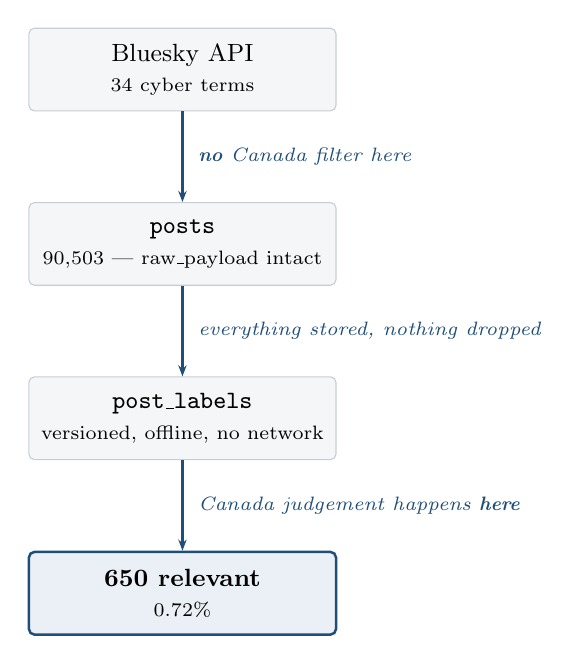
\begin{tikzpicture}[
  node distance=0pt,
  stage/.style={draw=rule, fill=softbg, rounded corners=2pt, minimum width=3.9cm,
                minimum height=1.05cm, align=center, font=\small},
  hl/.style={draw=accent, fill=accentbg, line width=0.9pt},
  lbl/.style={font=\scriptsize\itshape, text=accent, align=center},
  arr/.style={-{Stealth[length=4pt]}, draw=accent, line width=0.8pt}]

\node[stage] (api) {Bluesky API\\\scriptsize 34 cyber terms};
\node[stage, below=1.15cm of api] (posts) {\code{posts}\\\scriptsize 90{,}503 --- raw\_payload intact};
\node[stage, below=1.15cm of posts] (labels) {\code{post\_labels}\\\scriptsize versioned, offline, no network};
\node[stage, hl, below=1.15cm of labels] (rel) {\textbf{650 relevant}\\\scriptsize 0.72\%};

\draw[arr] (api) -- node[lbl,right=2pt]{\textbf{no} Canada filter here} (posts);
\draw[arr] (posts) -- node[lbl,right=2pt]{everything stored, nothing dropped} (labels);
\draw[arr] (labels) -- node[lbl,right=2pt]{Canada judgement happens \textbf{here}} (rel);
\end{tikzpicture}
\caption{Collection is deliberately broad; the Canada judgement happens downstream,
where it stays recomputable. 89{,}853 of the 90{,}503 collected posts are irrelevant
and are kept anyway.}
\label{fig:funnel}
\end{figure}

\textbf{Rationale --- a deliberate asymmetry in reversibility:}

\noindent
\begin{tabularx}{\textwidth}{@{}>{\raggedright\arraybackslash}p{0.33\textwidth} L@{}}
\toprule
 & \hd{If this judgment is wrong} \\
\midrule
Collection filter (cyber terms) & \textcolor{warn}{\textbf{Irreversible.}} Posts not fetched cannot be recovered. \\
Relevance filter (Canada terms) & \textcolor{good}{\textbf{Reversible.}} Raw payload is intact; recompute. \\
\bottomrule
\end{tabularx}

\vspace{0.6em}
Cybersecurity vocabulary is stable enough to serve as a collection boundary.
``What counts as Canada-related'' is precisely the definition most likely to
change --- so it belongs on the recomputable side.

\textbf{This was vindicated three times in one day.} Three separate errors were
found in the Canada rules, and \emph{none} required re-collection:

\noindent
\begin{tabularx}{\textwidth}{@{}L>{\raggedright\arraybackslash}p{0.42\textwidth}@{}}
\toprule
\hd{Discovery} & \hd{Impact} \\
\midrule
\code{GTA} $=$ \textbf{Grand Theft Auto}, not Greater Toronto Area &
  18.1\% of ``relevant'' was video-game news \\
\code{CRA} $=$ EU \textbf{Cyber Resilience Act}, not Canada Revenue Agency &
  part of a 15.4\% abbreviation error rate \\
\code{CSIS} $=$ csis.org, a \textbf{US think tank} & same \\
\bottomrule
\end{tabularx}

\vspace{0.6em}
Had ``canada'' been used as a \emph{search} term, these errors would have been
frozen into the corpus permanently --- the correctly-relevant posts that the
flawed query never retrieved simply would not exist to recover.

\textbf{The cost is 139$\times$ storage overhead.} 89{,}853 of 90{,}503 posts are
irrelevant and kept anyway. Disk is cheap; lost history is not.

A second-order consequence worth noting: this design means \textbf{the Canada
definition can be upgraded from rules to a classifier, or to entity linking,
without touching collection at all.} The rule-based labeler is a starting point,
not an architectural commitment.

\subsection{Why \texorpdfstring{\code{GTA}}{GTA} is instructive beyond its own fix}

The obvious fix for an ambiguous abbreviation is ``require cybersecurity context
nearby.'' That fix \textbf{does not work here}, and understanding why shaped the
final design.

\code{CRA}, \code{GRC}, \code{CSE}, \code{CSIS} are ambiguous \emph{between two
cybersecurity meanings}:

\begin{itemize}[leftmargin=1.4em,itemsep=0.15em]
\item \code{CRA} --- Canada Revenue Agency \textbf{vs.} EU Cyber Resilience Act
\item \code{GRC} --- Gendarmerie royale du Canada \textbf{vs.} Governance / Risk / Compliance
\item \code{CSIS} --- Canadian Security Intelligence Service \textbf{vs.} csis.org (US)
\end{itemize}

Requiring cyber context is satisfied by \emph{both} readings, so it discriminates
nothing. The working mechanism is \textbf{corroboration}: a weak abbreviation
only counts if an independent \emph{Canada-side} signal also fires. Implemented
as \code{requires\_corroboration} on weak abbreviation groups, with \code{RCMP}
kept as the sole strong abbreviation.

Measured effect: \code{is\_relevant} precision \textbf{56.0\% $\to$ 86.3\%},
recall \textbf{85.6\% $\to$ 91.7\%} (Section~\ref{sec:labeler}).

\subsection{Two collection modes, and why they are separate}
\label{sec:modes}

\begin{center}
\begin{tabularx}{\textwidth}{@{}>{\raggedright\arraybackslash}p{0.22\textwidth}
                               >{\raggedright\arraybackslash}X
                               >{\raggedright\arraybackslash}X@{}}
\toprule
 & \hd{\code{backfill}} & \hd{\code{incremental}} \\
\midrule
Cadence            & one-off, manual & \textbf{every 15 minutes} (cron) \\
Window per run     & a full history span (30 days used) & \textbf{30 minutes} \\
Internal structure & \textbf{chunked by day}, 34 terms per day & single window, 34 terms \\
Runs to date       & 6 & 72 \\
Mean collection lag& \textbf{354\,h} & \textbf{4\,h} \\
Mean likes observed& \textbf{3.59} & \textbf{1.50} \\
\bottomrule
\end{tabularx}
\end{center}

\vspace{0.4em}
\textbf{Why \code{incremental} exists:} the corpus accrues with wall-clock time.
A stopped collector loses that day permanently. This is the component that must
never stop.

\textbf{Why \code{backfill} exists:} trend detection compares two windows. With
7-day windows and only incremental collection, the first report would be
impossible until day 14. Backfill gives the trend layer a baseline on day 0. In
practice the first report was produced the same night collection started.

\textbf{Why day-chunking is mandatory, not an optimization:} \code{searchPosts}
returns results in reverse-chronological order and pages backwards. Once a page
limit is hit, \textbf{the truncated portion is always the older dates}. Paging
naively over a 30-day span systematically under-samples the past --- which
surfaces in the trend layer as a clean upward slope that is entirely an artifact
of collection. Day-chunking gives each day an independent page budget.
\emph{(Side benefit: process RSS dropped from 0.5\,GB to 4\,MB, because each
chunk flushes to the database.)}

\begin{warnbox}
\textbf{Why they are two modes rather than one mechanism:} their sampling
properties genuinely differ. The 2.4$\times$ gap in observed likes above is
\textbf{pure measurement artifact} --- \code{like\_count} is a snapshot taken at
collection time, and backfill posts had two weeks to accumulate engagement while
incremental posts had four hours. A system that did not distinguish the modes
would report ``last week was 2.4$\times$ more engaging'' as a social finding.
\code{collection\_runs.mode} makes the distinction auditable, and reports
disclose the mix.
\end{warnbox}

\textbf{Self-healing:} the incremental window is computed from the last
successful checkpoint, not from \code{now - 30min}. After a 10-hour outage, the
next run's window is automatically 10 hours wide. The 15-minute overlap
(deliberate, and harmless because \code{post\_uri} is a primary key) catches
posts that enter the search index late.

\subsection{Pipeline}

\begin{figure}[htbp]
\centering
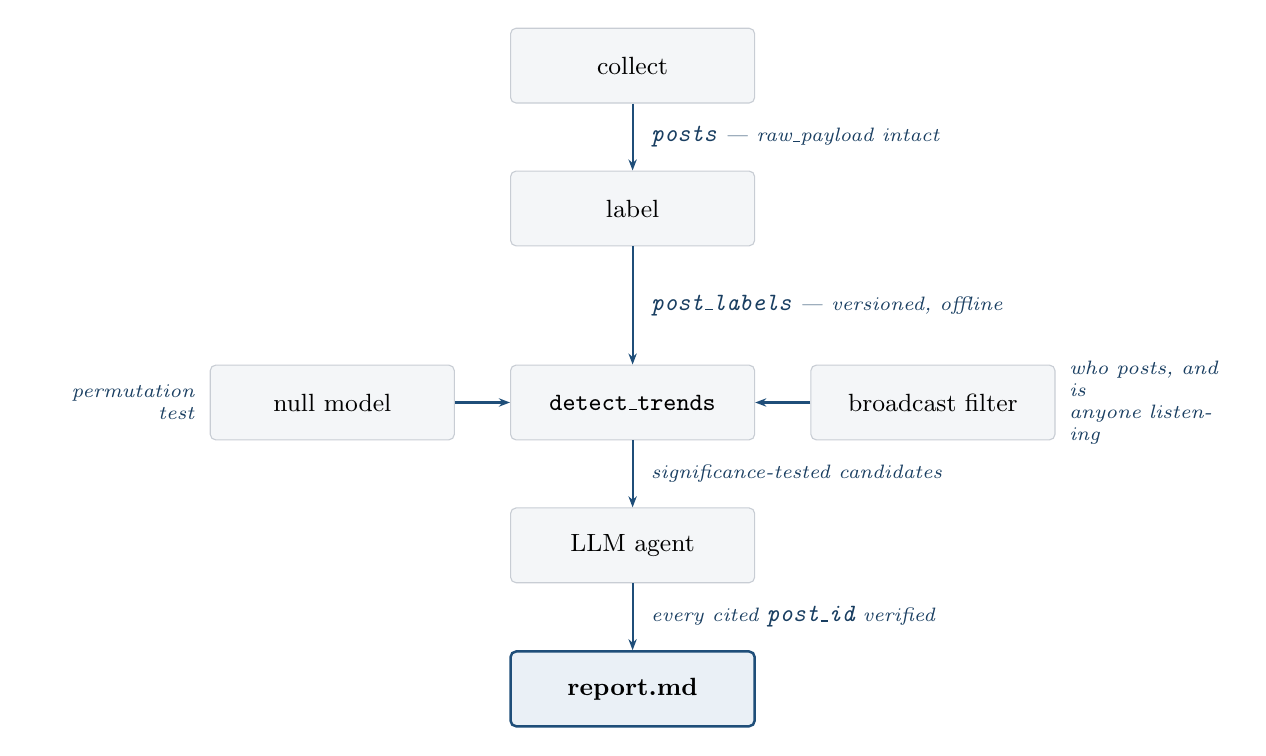
\begin{tikzpicture}[
  box/.style={draw=rule, fill=softbg, rounded corners=2pt, minimum height=0.95cm,
              minimum width=3.1cm, align=center, font=\small},
  outbox/.style={draw=accent, fill=accentbg, line width=0.9pt},
  note/.style={font=\scriptsize\itshape, text=accent!80!black, align=left},
  arr/.style={-{Stealth[length=4pt]}, draw=accent, line width=0.8pt}]

\node[box] (col) {collect};
\node[box, below=0.85cm of col] (lab) {label};
\node[box, below=1.5cm of lab] (trend) {\code{detect\_trends}};
\node[box, left=0.7cm of trend] (null) {null model};
\node[box, right=0.7cm of trend] (bc) {broadcast filter};
\node[box, below=0.85cm of trend] (agent) {LLM agent};
\node[box, outbox, below=0.85cm of agent] (rep) {\textbf{report.md}};

\draw[arr] (col) -- node[note,right=3pt]{\code{posts} --- raw\_payload intact} (lab);
\draw[arr] (lab) -- node[note,right=3pt]{\code{post\_labels} --- versioned, offline} (trend);
\draw[arr] (null) -- (trend);
\draw[arr] (bc) -- (trend);
\draw[arr] (trend) -- node[note,right=3pt]{significance-tested candidates} (agent);
\draw[arr] (agent) -- node[note,right=3pt]{every cited \code{post\_id} verified} (rep);

\node[note, left=2pt of null, text width=2.0cm, align=right]
  {permutation\\test};
\node[note, right=2pt of bc, text width=2.0cm]
  {who posts, and is\\anyone listening};
\end{tikzpicture}
\caption{End-to-end pipeline. Significance testing and the broadcast filter sit
\emph{between} trend detection and the agent, so the agent is never asked to
explain a change that the null model has already rejected.}
\label{fig:pipeline}
\end{figure}

\subsection{Implemented components}

\noindent
\begin{tabularx}{\textwidth}{@{}>{\raggedright\arraybackslash}p{0.21\textwidth} L@{}}
\toprule
\hd{Component} & \hd{What it does} \\
\midrule
\textbf{Collector} & AT Protocol XRPC; persistent session with \code{refreshJwt}; exponential backoff; rate-limit-aware; day-chunked backfill \\
\textbf{Ingest} & Idempotent upsert; run bookkeeping on an independent connection; stale-run reaping; timestamp repair \\
\textbf{Labeler} & Versioned rule engine; bilingual lexicons; cyber / Canada / topic classification; corroboration logic; negative guards \\
\textbf{Evaluation} & Stratified sampling, Wilson confidence intervals, precision/recall/F1 per label version \\
\textbf{Trend detection} & Adjacent-window comparison; posts \emph{and} unique authors; no composite score \\
\textbf{Null model} & Permutation test, two null hypotheses, family-wise error correction \\
\textbf{Broadcast filter} & Behavioral identification of automated feeds and promotional accounts \\
\textbf{Agent} & Anthropic or local OpenAI-compatible backend; 3 tools; structured output; hallucination verification \\
\textbf{Reporting} & Markdown with full provenance; data-health warnings; persisted to \code{analysis\_runs} \\
\textbf{Ops} & cron-driven collection; health check; log rotation; 191 tests \\
\bottomrule
\end{tabularx}

% ===========================================================================
\section{Findings}

\subsection{The labeler was substantially wrong, and this was measurable}
\label{sec:labeler}

A 100-post stratified sample was drawn across four strata (relevant /
cyber-only / Canada-only / neither); 99 of 100 were annotated. Scores are
stratum-weighted with Wilson confidence intervals.

\begin{center}
\begin{tabular}{@{}lrr@{}}
\toprule
\hd{Metric} & \hd{\code{rules\_v1}} & \hd{\code{rules\_v2}} \\
\midrule
\code{is\_relevant} \textbf{precision} & \textbf{56.0\%} & \textbf{86.3\%} \\
\code{is\_relevant} \textbf{recall}    & 85.6\% & \textbf{91.7\%} \\
F1 & 67.7\% & \textbf{88.9\%} \\
\bottomrule
\end{tabular}
\end{center}

\begin{warnbox}
\textbf{Nearly half of what v0 called ``Canada-related cybersecurity
discussion'' was not.} The headline pilot number was revised from 27/day to
\textbf{21.3/day}.
\end{warnbox}

This matters methodologically more than numerically: \textbf{v0 reported a number
it had never validated.} Everything downstream inherited a 44\% false-positive
rate silently. The fix was not a better rule --- it was \emph{measuring the rule
at all}.

\subsection{No topic in the current window is distinguishable from noise}
\label{sec:noise}

v0's trend detection answered ``which topic changed most.'' It could not answer
``is that change larger than random fluctuation.'' A permutation test was added
to close that gap.

\begin{center}
\begin{tabular}{@{}lrrrrl@{}}
\toprule
\hd{topic} & \hd{$\Delta$} & \hd{growth} & \hd{null sd} & \hd{p (FWER)} & \hd{verdict} \\
\midrule
\code{data\_breach}         & $+10$ & $+56\%$  & 7.45  & \textbf{0.718} & \noise \\
\code{other}                & $+4$  & $+5\%$   & 13.84 & 0.991 & \noise \\
\code{malware\_infostealer} & $+3$  & $+100\%$ & 3.29  & 0.998 & \noise \\
\code{fraud\_financial}     & $+2$  & $+22\%$  & 4.69  & 1.000 & \noise \\
\code{ransomware}           & $-5$  & $-20\%$  & 7.47  & 0.969 & \noise \\
\bottomrule
\end{tabular}
\end{center}

\begin{keybox}
\textbf{Under the null hypothesis, random fluctuation alone produces a swing of
$\pm28$ in \emph{some} topic. The largest observed change is $+10$.}
\end{keybox}

Two null models are implemented:

\begin{description}[leftmargin=1.4em,style=nextline,itemsep=0.35em]
\item[post-level] Reshuffle window assignment per post. Ignores author
  clustering, so its $p$-values are optimistic. Kept as a comparison baseline.
\item[author-level (default)] Circularly shift each author's \emph{entire}
  posting history by a whole number of days across the 14-day span. This
  preserves each author's post count, topic mix, and burst structure, and
  destroys only the alignment between author activity and the calendar. It rules
  out the explanation \emph{``this topic rose because a few prolific accounts
  happened to cluster.''}
\end{description}

The author-level null distribution is about 20\% wider than the post-level one
(\code{other}: sd $8.52 \to 13.84$), confirming the corpus is over-dispersed.

\textbf{Multiple comparisons are corrected.} Choosing the largest of 10 topics to
narrate is a textbook look-elsewhere effect. Each permutation additionally
records the maximum $|\Delta|$ across all topics, giving a family-wise corrected
$p$-value via the max-statistic method.

\subsubsection*{Why $z$-scores were rejected}

The v1 specification called for $z$-score-based detection. This was tested and
rejected on evidence:

\begin{warnbox}
Real corpus $\max|z|$ ranges \textbf{0.2--0.9}. Pure Poisson noise produces
$|z|$ with a \textbf{median of 1.4--1.7} and a \textbf{95th percentile of
3.0--4.0}.
\end{warnbox}

\textbf{The $z$-score scores noise higher than it scores the real data.} It is
anti-informative at this volume. The cause is that the Poisson variance
assumption fails: one author posting eight times, or a single news item being
widely reshared, breaks independence. Permutation testing makes no
distributional assumption and is therefore valid where the $z$-score is not.

\subsection{How much more data would be needed: about 8\texorpdfstring{$\times$}{x}}
\label{sec:power}

Rather than assuming $\sqrt{n}$ scaling, it was measured --- by replicating the
author pool $k$ times and re-running the permutation test.

\begin{center}
\begin{tabular}{@{}rrrrc@{}}
\toprule
\hd{scale $k$} & \hd{relevant / window} & \hd{null $\max|\Delta|$ p95} &
\hd{scaled $\Delta$} & \hd{detectable} \\
\midrule
1 & 158 & 28.0 & 10 & \no \\
2 & 316 & 40.0 & 20 & \no \\
4 & 632 & 56.0 & 40 & \no \\
\textbf{8} & \textbf{1{,}264} & \textbf{78.0} & \textbf{80} & \yes \\
16 & 2{,}528 & 108.0 & 160 & \yes \\
\bottomrule
\end{tabular}
\end{center}

Observed scaling matches $\sqrt{k}$. \textbf{An effect of the currently observed
size needs roughly 8$\times$ the data to become detectable}, reachable either by:

\begin{itemize}[leftmargin=1.4em,itemsep=0.15em]
\item lengthening windows to about 56 days (roughly 4 months of total span), or
\item increasing collection volume about 8$\times$ (more terms, more platforms).
\end{itemize}

This is the quantitative form of a concern that had previously only been
expressible as ``the data might not be enough.'' It is a $\sqrt{n}$ problem; no
amount of parameter tuning resolves it.

\subsection{A quarter of the corpus has no audience}
\label{sec:broadcast}

\begin{center}
\begin{tabular}{@{}lr@{}}
\toprule
Broadcast accounts & \textbf{11 of 372 (3.0\%)} \\
Posts they contribute & \textbf{158 of 650 (24.3\%)} \\
Their mean engagement & \textbf{0.20} \\
Everyone else's mean engagement & \textbf{5.34} \\
\bottomrule
\end{tabular}
\end{center}

They are two kinds of account:

\begin{enumerate}[leftmargin=1.6em,itemsep=0.2em]
\item \textbf{Automated threat-intelligence feeds} --- \code{ecrime.ch},
  \code{cyberintelligence.bsky.social}, \code{ransomlook.bsky.social},
  \code{falconfeedsio.bsky.social}. Ransomware leak-site monitors that auto-post
  every new victim.
\item \textbf{Security conference promotion} --- \code{bsidesedmonton.bsky.social},
  \code{hackfest.bsky.social}. Repeated CFP and event announcements.
\end{enumerate}

\textbf{Neither is public discussion.} Counting them toward topic volume means
measuring a bot's posting rate and calling it social attention.

\begin{keybox}
\textbf{The concrete damage:} of 45 \code{ransomware} posts in 14 days,
\textbf{40 came from 5 automated feeds} (4.5 posts/author, versus 1.0--1.4 for
every other topic). Excluding them removes \code{ransomware} from the trend
ranking entirely. Every \code{ransomware} rise or fall in earlier reports was
measuring feed uptime.
\end{keybox}

Detection is \textbf{behavioral, not a handle blocklist} --- blocklists rot and
do not transfer across time windows:

\begin{center}
\code{n\_posts} $\geq$ 5 \quad\textbf{and}\quad
\code{n\_active\_days} $\geq$ 4 \quad\textbf{and}\quad
zero-engagement rate $\geq$ 60\%
\end{center}

\textbf{A trap that had to be avoided here:} \code{like\_count} is a snapshot
taken at collection time. Incremental collection captures posts about 4 hours
old; backfill averaged 354 hours. Without a guard, ``zero engagement'' would
classify \emph{every freshly collected post} as a bot. The zero-engagement rate
therefore only counts posts with $\geq 24$\,h of settling time. The confound was
then checked directly and does not drive the result --- broadcast accounts
actually have \emph{longer} collection lag (359\,h vs 323\,h), and restricting
to posts with $>168$\,h of settling preserves the gap (76.7\% vs 50.0\%
zero-engagement; 0.19 vs 3.15 mean likes). The guard stays regardless, because
the next dataset may not be so forgiving.

\subsection{The agent separates two questions that are easy to conflate}

When the null model returns \noise, the system automatically switches the
agent's prompt. The original prompt opened with \emph{``the statistical layer has
determined this is the top candidate trend; your task is to explain it''} ---
which, applied to a change indistinguishable from noise, is an instruction to
confabulate.

The replacement prompt asks a different question: \emph{``setting volume aside
entirely, is there a coherent story in these posts or not?''} --- and states
explicitly that ``no, there is no story'' is a correct and valuable answer.

It forces a verdict on two \textbf{independent} axes:

\begin{center}
\begin{tabularx}{0.92\textwidth}{@{}>{\raggedright\arraybackslash}p{0.30\textwidth} L@{}}
\toprule
\hd{field} & \hd{this window} \\
\midrule
\code{trend\_claim\_supported} & \code{not\_supported} --- the volume rise does not hold up \\
\code{coherence} & \code{one\_story} --- but the content genuinely is one event \\
\bottomrule
\end{tabularx}
\end{center}

\begin{keybox}
\textbf{These do not contradict each other}, and the distinction is the useful
output: there is a real incident in the posts (an Alberta voter-list breach),
but its effect on volume is indistinguishable from noise. \emph{The event is
reportable; ``it is trending'' is not.}
\end{keybox}

Evidence integrity is enforced mechanically: every \code{post\_id} the agent
cites is checked against the set of posts the tools actually returned.
Hallucinated IDs are not silently dropped --- they are flagged in the published
report, so readers can judge that run's reliability. In the current run, all 5
cited IDs verified, and the agent additionally flagged 2 of them as belonging to
a \emph{different} incident under the same topic label.

% ===========================================================================
\section{Limitations}

\subsection{Known and unresolved}

\begin{description}[leftmargin=1.4em,style=nextline,itemsep=0.45em]
\item[Single source.] Bluesky only. Not representative of Canadian discourse,
  and the size of that gap is unmeasured. This is the largest limitation and it
  is structural.

\item[Volume is about 8$\times$ short] of detecting trends of the observed
  magnitude (Section~\ref{sec:power}). The system currently produces defensible
  \emph{descriptions} of a window and defensible \emph{negative} results. It
  cannot yet produce positive trend claims.

\item[The evaluation set has an independence problem.] The gold set was
  annotated by the same agent that wrote the labeler being evaluated. Systematic
  blind spots in the rules are likely to be reproduced in the annotations, which
  would inflate both precision and recall. \emph{Independent annotation by a
  domain expert is the highest-value next step for validity}, and it is cheap
  --- it is one TSV file.

\item[The evaluation set covers only backfill data.] All 99 labeled samples came
  from backfill collection. Incremental data --- which differs systematically in
  collection lag and observed engagement --- is unevaluated.

\item[\code{other} absorbs about 44\% of relevant posts.] The topic lexicon does
  not cover nearly half the corpus, which limits what cross-topic comparison can
  mean.

\item[Strong weekday effect.] Weekend volume is about 45\% of weekday volume
  (roughly 15 vs 33 relevant/day). Any window shorter than 7 days, or any
  comparison where the two windows contain different numbers of weekends, is
  badly confounded. The 14-day / 2-window design balances this by construction,
  but it constrains window choice.

\item[Engagement metrics are snapshots, not final values]
  (Section~\ref{sec:modes}). Cross-mode engagement comparison is invalid without
  a correction that does not yet exist.

\item[French coverage is thin.] 22 of 650 relevant posts. Measured cause: French
  technical vocabulary is largely unused in practice --- \code{rançongiciel}
  returned 1 post in 7 days, \code{hameçonnage} 5, while \code{cybersécurité}
  returned hundreds. The Canada lexicon therefore carries French signal through
  place and institution names rather than translated jargon. Whether this
  under-represents Francophone discussion or accurately reflects it is
  \textbf{not currently known}.

\item[Rule-based relevance.] 86.3\% precision means roughly one in seven
  ``relevant'' posts is not. Entity linking or a trained classifier would be
  better; the versioned-labels design (P2) means either can be added without
  re-collection.
\end{description}

\subsection{Explicitly out of scope}

Sentiment analysis, embeddings and semantic drift, entity extraction, named
network analysis, Prometheus/Grafana, real-time alerting, a web UI. These were
deferred deliberately --- not for effort reasons, but because \textbf{the corpus
cannot currently support conclusions drawn from them}, and building them would
manufacture confidence rather than knowledge.

\subsection{Ethical and legal posture}

Collection uses the documented public API under its terms of service, with
authenticated access at about 1\% of the published rate limit. Only public posts
are collected. No attempt is made to deanonymize, aggregate profiles, or track
individuals; author identifiers exist solely to detect posting concentration,
which is a methodological control (Section~\ref{sec:broadcast}), not a subject of
study. A request to create synthetic accounts to expand access was declined as a
terms-of-service violation.

% ===========================================================================
\section{Implementation notes --- what broke and what it taught}
\label{sec:incidents}

Every item below was found by the system's own instrumentation rather than by
inspection, which is the argument for principles P3 and P5.

\begin{center}
\small
\begin{tabularx}{\textwidth}{@{}>{\raggedright\arraybackslash}p{0.20\textwidth} L L@{}}
\toprule
\hd{Incident} & \hd{Root cause} & \hd{Consequence if undetected} \\
\midrule
\textbf{10h23m collection outage} &
  Bluesky returns \textbf{HTTP 400} with \code{\{"error":"ExpiredToken"\}} for
  expired tokens, not 401. The refresh path only triggered on 401. &
  A 10-hour hole in the time series, visually identical to a drop in discussion \\
\textbf{Reverse-pagination truncation} &
  Search returns newest-first; page limits always truncate the oldest dates &
  A fabricated upward trend across the entire backfill period \\
\textbf{\code{createdAt} is client-supplied} &
  53 posts backdated $>$2 days (one to 2016), 238 future-dated &
  Posts landing in the wrong analysis window \\
\textbf{Inherited \code{America/Toronto} timezone} &
  New cluster inherits host timezone; \code{date\_trunc} depends on session TZ &
  23- and 25-hour days across DST; silently wrong daily counts \\
\textbf{NUL byte crash} &
  PostgreSQL cannot store U+0000; a post contained one &
  Killed a backfill run after 52{,}079 posts \\
\textbf{\code{partial} status too coarse} &
  Any HTTP error marked the run partial; token refresh happens roughly every 2h &
  Every run flagged \code{partial}, drowning the P5 signal entirely \\
\textbf{Stale \code{running} runs} &
  \code{SIGKILL} bypasses exception handlers &
  Permanently open run records \\
\textbf{Duplicate CLI command registration} &
  Two \code{analyze} definitions; the later silently shadowed the earlier &
  Edits applied to dead code \\
\bottomrule
\end{tabularx}
\end{center}

\vspace{0.6em}
\begin{warnbox}
\textbf{The outage is the most instructive.} A test named
\code{test\_401\_refreshes\_without\_new\_login} existed and passed. It tested
\emph{the error shape I had imagined}, not the one the API actually produces.
The refresh token was valid for another three months and was never called. The
lesson is narrow and transferable: \textbf{a test written against an assumed
contract validates the assumption, not the integration.} The fix now matches on
the error body across both status codes, with four regression tests derived from
captured real responses.
\end{warnbox}

% ===========================================================================
\section{What I would do next, in priority order}
\label{sec:next}

\begin{enumerate}[leftmargin=1.6em,itemsep=0.35em]
\item \textbf{Independent annotation of the evaluation set.} Cheapest available
  improvement to validity, and it currently gates the credibility of every
  precision/recall number in this document.
\item \textbf{Add Reddit as a second source.} Directly attacks the two largest
  limitations at once --- single-source bias and the 8$\times$ volume shortfall
  --- and Reddit is discussion-shaped rather than broadcast-shaped, which
  Section~\ref{sec:broadcast} suggests matters a great deal.
\item \textbf{Extend the evaluation set to incremental data}, so the labeler is
  validated on both sampling regimes rather than one.
\item \textbf{Longer windows (28--56 days) once the corpus supports them}, per
  the power analysis. Slower-moving, but actually detectable.
\item \textbf{Correct engagement for collection lag}, enabling valid cross-mode
  comparison and a better-grounded broadcast filter.
\item \textbf{Only then} revisit entities, keywords, and semantic drift --- once
  there is enough data for them to mean something.
\end{enumerate}

% ===========================================================================
\section{Repository guide}

\noindent
\begin{tabularx}{\textwidth}{@{}>{\raggedright\arraybackslash}p{0.33\textwidth} L@{}}
\toprule
\hd{Path} & \hd{Contents} \\
\midrule
\code{HANDOFF.md} & v0 specification \\
\code{TREND\_AGENT.md} & v1 specification (trend analysis agent) \\
\code{README.md} & Implementation detail, measured API behavior, decision records, full findings \\
\code{PROJECT\_WRAPUP.md} & This document (Markdown source) \\
\code{reports/wave1\_all.md} & First-wave analysis, full corpus \\
\code{reports/\allowbreak wave1\_no\_broadcast.md} & First-wave analysis, broadcast accounts excluded \\
\code{eval/sample.tsv} & 100-post annotated evaluation set \\
\code{src/ccint/collectors/} & Bluesky AT Protocol client \\
\code{src/ccint/labelers/} & Versioned rule engine + bilingual lexicons \\
\code{src/ccint/analytics/} & Trend detection, null model, broadcast filter \\
\code{src/ccint/agent/} & Tool definitions, prompts, analysis loop \\
\code{migrations/} & Numbered SQL migrations \\
\code{tests/} & 191 tests \\
\bottomrule
\end{tabularx}

\begin{shell}
ccint collect backfill --since 2026-08-22    # seed history
ccint collect incremental                    # cron, every 15 min
ccint label --version rules_v2               # offline, recomputable
ccint eval score                             # precision / recall / F1
ccint analyze --window 7 --null-iter 5000 --exclude-broadcast
\end{shell}

% ===========================================================================
\section*{Closing note}
\addcontentsline{toc}{section}{Closing note}

\begin{keybox}
The most useful thing this project produced is \textbf{the ability to tell that
it has not found a trend.}
\end{keybox}

A version of this system that reported \code{data\_breach} $+56\%$ would look
more successful and would be wrong. The layers that produce the negative result
--- the null model, the power analysis, the broadcast filter, the evaluation
set, the prompt that permits the agent to say ``there is no story here'' --- are
the actual deliverable. The corpus will grow; the discipline to know when it is
large enough has to be built first.

\end{document}
